\chapter{Transport Layer Security}
TLS, or Transport Layer Security, was originally proposed by Netscape
in 1995 as a way to secure communications between a web browser and a
web server. It is the successor to SSL, or Secure Sockets Layer, which
was first introduced by Netscape in 1995. The two terms are often used
interchangeably, but TLS is the more modern and secure protocol.\\ 
The main goal of SSL was to create secure network channel, almost at
session level(4.5), between two parties, to provide some security
services that neither TCP nor IP provides:
\begin{itemize}
  \item \textbf{peer authentication} based on asymmetric
    challenge-response authentication(the challenge for the service is
    implicit, while for the client is explicit). Server authentication
    is alway compulsory, while client authentication is optional and
    requested by the server.
  \item \textbf{message confidentiality} base on symmetric encryption
  \item \textbf{message integrity} and authentication based on MAC
    computed on the trasmitted data
  \item \textbf{replay, filtering and reordering attack protection}
    using implicit record numbers( the correct order of transmission
    is provided by TCP, for this reason the number is implicit). This
    number is used also in the MAC computation.

\end{itemize}

You can see the TLS packet structure in figure
\ref{fig:tls-packet-structure}.
The TLS handshake protocol is used to establish a new session or 
reestablish an existing session. The TLS change cipher spec protocol 
is used to trigger the change of the algorithms to be used for message 
protection, or most notably to pass from the previous unprotected 
session to a protected one. The TLS alert protocol is used to signal
errors or signal the end of the connection. 
The TLS record protocol contains the generic protocols informations
and its content depend of the state of the connection and the protocol
it is tunneling.
\begin{figure}[H]
    \centering
    \includegraphics[width=.6\textwidth]{img/TLS packet
    structure.png}
    \caption{TLS packet structure.}
    \label{fig:tls-packet-structure}
\end{figure}

\section{TLS session and connection}
It is important to make a clear distinction between TLS session and
connections.\\
\textbf{TLS sessions} a \textbf{logical association} between client and server, created
via an handshake protocol and its shared between different TLS
connections(1:N).\\
\textbf{TLS connections} are a \textbf{transient TLS channel} between client and server,
which means that each connection is associated with only one specific
TLS session(1:1).

\begin{figure}[H]
  \centering
  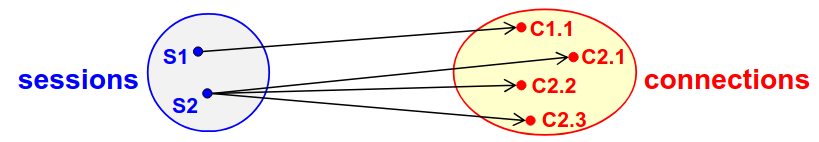
\includegraphics[width=.7\textwidth]{img/TLS session connection.png}
  \caption{TLS session and connection.}
  \label{fig:tls-session-and-connection}
\end{figure}
\section{TLS handshake protocol}
The TLS handshake protocol is used to establish a new session or
reestablish an existing session. It's a critical part of the TLS
protocol, because the channel pass from an unprotected state to a
protected one. During this phase the two parts agree
agree on a set of algorithms for confidentiality and integrity,
exchange random numbers between the client and the server to be used
for the subsequent generation of the keys, establish a symmetric key
by means of public key operations (originally RSA and DHKE, but
nowadays the elliptic curve versions of algorithms are used) and negotiate the
session-id and exchange the necessary public keys certificates for the
asymmetric challenge-response authentication.

\section{Achieving Data protection}
Data protection is achieved by using symmetric encryption algorithms
to encrypt the data and Message Authentication Codes(MAC) to ensure
the integrity of the data and the authentication of the sender.\\
Figure \ref{fig:tls-data-protection} shows how the data protection is 
achived in TLS using authenticate-then-encrypt approachm, but also
encrypt-then-authenticate is possible.\\
The MAC is computed over the data(compressed or not), the TLS sequence 
number and the key used for the MAC computation. The padding is also
part of the MAC computation to avoid those attacks that change the
padding.\\
The MAC is then encrypted with the dedicated symmetric key and a
suitable initialization vector(IV) 

\begin{figure}[H]
  \centering
  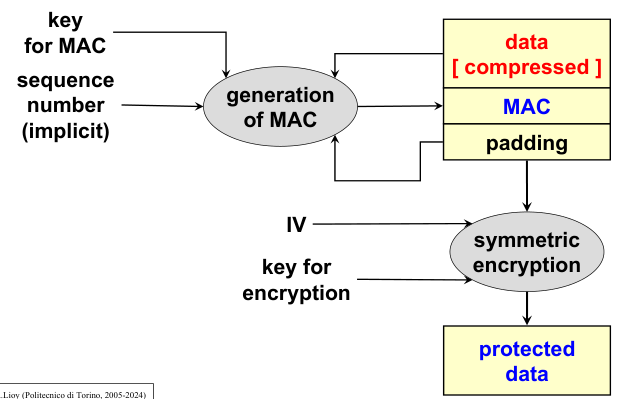
\includegraphics[width=.5\textwidth]{img/TLS data protection.png}
  \caption{TLS data protection.}
  \label{fig:tls-data-protection}
\end{figure}

The keys are \textbf{directional}, so there are two keys( one for
client to server and one for server to client) to protect against
reuse of the sequence number in the opposite direction.

\section{Relationship among keys and sessions}
When a new session is created using the handshake protocol, a new
\textbf{pre-master secret} is established using public key
cryptography. Then from the session a new connection is created, which
requires a random number to be generated, and exchanged between the
client and the server. Those two values are combined via a KDF,
usually HHKDF( HMAC-based key derivation function) to generate the 
\textbf{master secret}. This computation is done only once, and the 
secret is common to several connections.\\
The pre-master secret is then discarded, and the keys necessary for
the MAC computation, encryption and, if necessary, IVs will be derived
from the master secret.\\
You can notice that the master secret is common to any connections
inside a session, but the per-connection keys are different every
time. This is another important feature to avoid replay attacks,
possible because numbering is per-connection. This solution also
allows to reduce the cost of establishing new keys for each
connection.

\begin{figure}[H]
  \centering
  \includegraphics[width=.5\textwidth]{img/relationship
  keys-connection.png}
  \caption{Relationship among keys and sessions.}
  \label{fig:tls-keys-and-sessions}
\end{figure}

\section{Perfect Forward Secrecy}
Since the keys are generated from symmetric crypto, if the private key
used to perform encryption and decryption of the pre-master secret is
compromised, all the previous communication can be decrypted because
it is possible to derive the master-secret. This is only possible if
the server has a certificate valid for both signature and encryption
In this context, perfect forward secrecy is desirable.
\begin{boxH}
  \textbf{Perfect Forward Secrecy} is a property of key-agreement
  protocols ensuring that the compromise of the secret key used for 
  will compromise only current (and eventually future) traffic but not
  the past one
\end{boxH}
The most common way to achieve this is to use \textbf{ephemeral keys},
which are one-time asymmetric keys( used for key exchange). This means
that the key pair used for key exchange is not a long term key pair,
but a temporary one generated on-the-fly when necessary.\\ 
The ephemeral key needs to be authenticated, so only for this purpose
the long-term key is used for signing the ephemeral key. This is done
using DHKE instead of RSA because the latter one is really slow, while
the former one is faster with the compromise of only using the
established key for a certain number of session.\\
Let's now go over some considerations: if the temporary key is
compromised, perfect forward secrecy of the communication is still
valid because he can only decrypt the traffic exchanged using the
temporary key. On the contrary, if the long-term key is compromised,
no secret is really disclosed, because no traffic has been exchanged
using it for encryption, but is still a problem for server
authentication.

\section{The protocol}
The TLS handshake is always initiated by the client. 

\subsection{Client Hello and Server Hello}
In version 1.2 the client sends a \textbf{Client Hello}, which
contains:
\begin{itemize}
  \item the SSL version preferred by the client, and the highest
    supported(2=SSL-2, 3.0=SSL-3, 3.1=TLS-1.0, \dots)
  \item a 28 bytes pseudo-random number, which is the client random
  \item a session-id, which is \textit{0} if the client is starting a
    new session, and \textit{1} if the client is trying to resume a
    previous session
  \item a list of cipher suites supported by the client, in order to 
    let the server choose the most secure one (the set of algorithms
    used for encryption, for key exchange, and for integrity)
  \item a list of compression methods supported by the client
    (supported only up to TLS 1.2)
\end{itemize}

And then a \textbf{server hello} is sent back, which contains:
\begin{itemize}
  \item the SSL version chosen by the server, the highest one
    supported by both the client and the server
  \item a 28 bytes pseudo-random number, which is the server random
  \item a session identifier(session-id), which is a new one if the
    server is starting a new session, and the same as the client's if
    the server is resuming a previous session
  \item the cipher suite chosen by the server, the strongest common
    one between the client and the server
  \item the compression method chosen by the server
\end{itemize}


\begin{figure}[H]
  \centering
  \begin{subfigure}{.5\textwidth}
    \centering
    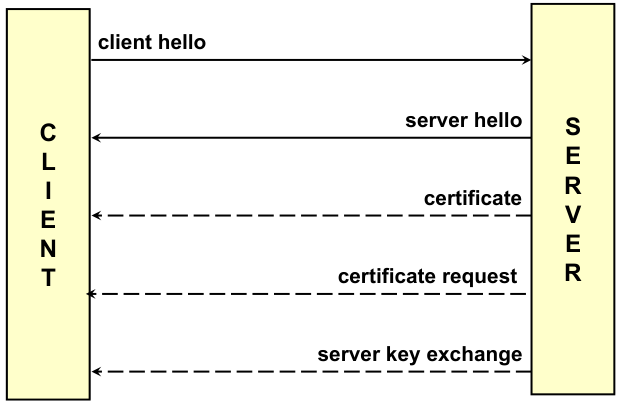
\includegraphics[width=.9\linewidth]{img/TLS key echange.png}
    \caption{The TLS handshake protocol(TLS 1.2).}
    \label{fig:tls-handshake-protocol-1.2}
  \end{subfigure}%
  \begin{subfigure}{.5\textwidth}
    \centering
    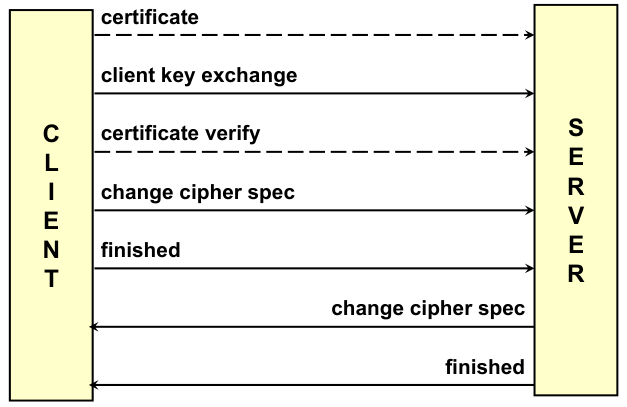
\includegraphics[width=.9\linewidth]{img/TLS key exchange 1-3.png}
    \caption{The TLS handshake protocol(TLS 1.3).}
    \label{fig:tls-handshake-protocol-1.3}
  \end{subfigure}
\end{figure}

\subsection{Cipher suite}
A cipher suite is a string which contains the set of cryptographic
algorithms used in the TLS protocol. A typical cipher suite consists
of a key exchange algorithm, the symmetric encryption algorithm, and
the hash function used for generating MACs.
Some example of those are:
\begin{itemize}
  \item SSL\_NULL\_WITH\_NULL\_NULL (no protection, used for the record
    protocol to be used in the handshake)
  \item SSL\_RSA\_WITH\_NULL\_SHA
  \item SSL\_RSA\_EXPORT\_WITH\_RC2\_CBC\_40\_MD5
  \item SSL\_RSA\_WITH\_3DES\_EDE\_CBC\_SHA
\end{itemize}


\subsection{Certificates}
After the initial exchange, the server is ready to authenticate
itself.\\
The server sends its long-term public key certificate to the client
for server authentication. Actually, the whole certificate chain, up
to the root CA, must be sent. Furthermore , the subject of the 
certificate must match the server name.\\
Server authentication is implicit, because its private key is used to
decrypt the pre-master secret, while client authentication is 
always explicit.

\begin{boxH}
  The implicit server authentication is based on the fact that the MAC
  is computed trough the key derived trough knowledge of the private
  key, so only the server can compute it.
\end{boxH}

Optionally, the server can request a certificate from the client for
client authentication. In this case the server specifies the list of
trusted CA's, and the client sends its certificate chain. The browsers
show to the users (for a connection) only the certificates issued by
trusted CAs.
If client certificate verification is required, an explicit request to
send the hash computed over all the handshake messages before this 
one and encrypted with the client private key is sent to the client.

\subsection{Key exchange}
The key exchange is the most important part of the handshake protocol.
If the server is using RSA for key exchange, the client generates a
pre-master secret, encrypts it with the server's public key(which can
be ephemeral or from its x.509 certificate) and sends it to the
server. If RSA is no used, DHKE can be used to generate the pre-master
secret, and in this case the server computes the value independently 
and the two parts can derive the master secret.\\
Another option is to use FORTEZZA, which is a key exchange algorithm
based on DH.

\subsection{Certificate verify}
In case the server requested client authentication, the client will be
required to send the certificate to prove that he is the owner of it's
private key. The message to be signed is the hash of all the messages
exchanged up to this point in the handshake protocol. This is to avoid
replay attacks too.


\subsection{Change cipher spec}
The change cipher spec message used to trigger the change of the
algorithms to be used for message protection. It allows to pass from
the previous unprotected messages to the protection of the next
messages with algorithms and keys just negotiated, thus is technically
a protocol on its own and not part of the handshake. Some analysis
even say that it could be removed from it.


\subsection{Finished message}
The finished message is the last message of the handshake protocol,
and the first message protected by the negotiated keys and algorithms.
It is necessary to ensure that the handshake has not been tampered
with, and it contains contains a MAC computed over all the previous
handshake messages (but change cipher spec) using as a key the master
secret. Notice that the finished message is different for the client 
and the server, because the MAC is computed over different messages.

This allows to prevent rollback man-in-the-middle attacks (version
downgrade or ciphersuite downgrade)

% 3 subfig, 2 on top and 1 on bottom
\begin{figure}[H]
  \centering
  \begin{subfigure}{.5\textwidth}
    \centering
    \includegraphics[width=.9\linewidth]{img/TLS no ephimeral no
    auth.png}
    \caption{TLS handshake(no ephemeral, no client authN).}
    \label{fig:tls-handshake-protocol}
  \end{subfigure}%
  \begin{subfigure}{.5\textwidth}
    \centering
    \includegraphics[width=.9\linewidth]{img/TLS no ephimeral
    auth.png}
    \caption{TLS handshake(no ephemeral, client authN).}
    \label{fig:tls-handshake-protocol-2}
  \end{subfigure}
  \begin{subfigure}{.5\textwidth}
    \centering
    \includegraphics[width=.9\linewidth]{img/TLS ephimeral no
    auth.png}
    \caption{TLS handshake(ephemeral, no client authN).}
    \label{fig:tls-handshake-protocol-3}
  \end{subfigure}
  \caption{TLS handshake protocol.}
\end{figure}

\section{Setup Time}
The setup time is the time required to establish a secure connection 
between the client and the server. TLS depends on TCP, so the TCP
handshake must be taken into account. Then the TLS handshake is
performed, meaning that typically 3 RTTs (1 for TCP and 2 for TLS) are
required to establish a secure connection. Usually after 180ms the two
parties are ready to send protected data( assuming 30ms delay
one-way).

% 2 subfig
\begin{figure}[H]
  \centering
  \begin{subfigure}{.5\textwidth}
    \centering
    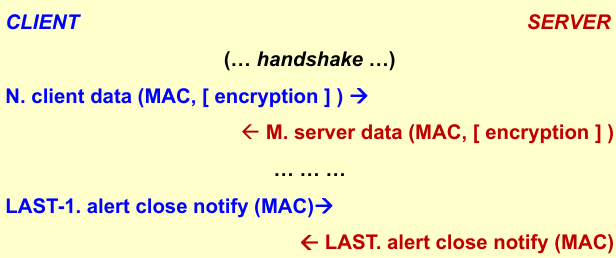
\includegraphics[width=.9\linewidth]{img/TLS link teardown.png}
    \caption{TLS link teardown.}  
    \label{fig:tls-link-teardown}
  \end{subfigure}%
  \begin{subfigure}{.5\textwidth}
    \centering
    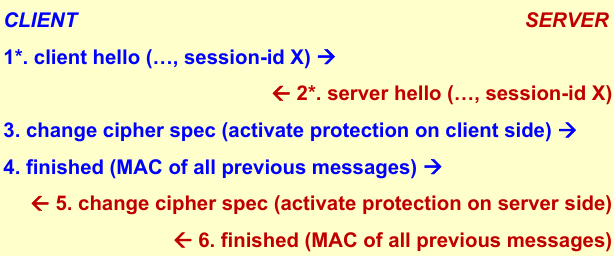
\includegraphics[width=.9\linewidth]{img/TLS resume session.png}
    \caption{TLS resume session.}
    \label{fig:tls-resume-session}
  \end{subfigure}
  \caption{TLS link teardown and resume session.}
\end{figure}

\section{TLS versions}
\subsection{TLS 1.0}
TLS 1.0, or SSL 3.1, was released in 1999. It is the first version of
the protocol, and it is based on SSL 3.0. Previous version were using
proprietary solutions, so the adoption of open standards was strongly
encouraged.

\subsection{TLS 1.1}
TLS 1.1 was released in 2006, and it introduced some security fixes
especially to protect against CBC attacks. In fact, the implicit
IV is replaced with an explicit IV to protect against CBC attacks.
Also protection against padding oracle attacks were introduces to
reduce the information leaks. For this reason Passing errors now use
the bad\_record\_mac alert message (rather than the decryption\_failed
one). Furthermore, premature closes no longer cause a session to be non-
resumable.

\subsection{TLS 1.2}
TLS 1.2 was released in 2008, and it introduced some new features and 
improvements. The chipersuite also specifies the pseudo random
function instead of leaving the choice to the implementation. The
sha-1 algorithm was replaced with SHA-256, and its also added support
for authenticated encryption, such as AES in GCN or CCM mode.

All the chipersuites tat use IDEA and DES are deprecated.

\section{TLS attacks}
\subsection{Heartbleed}
Heartbleed is a security bug in the OpenSSL cryptography library,
which is a widely used implementation of the TLS protocol. It was able
to exploit the fact that the heartbeat extension keeps the connection
alive without the need to negotiate the SSL session again. The
attacker could send a heartbeat request, but the length of the 
response is much longer( up to 64KB) than the actual data sent by the
client. This attack could then allow to leak memory contents.

\subsection{Bleichenbacher attack}
Blackenbacker is a 1998 attack and it's the so-called the million
message attack because it exploited a vulnerability in the way the RSA
encryption was done. RSA requires the padding to be done in a certain
way, because if it is unoptimally done, it could cause some issues.\\
The attacker could perform an RSA private key operation with a
server’s private key by sending a million or so well-crafted messages
and looking for differences in the error codes returned. By basically
knowing the public key and trying to decrypt a message with some
guessed private keys, the different responses obtained were giving
hints about which bits were correct and which bits were wrong.\\
Later one the RSA implementations moved to RSA-OAEP, which is a
padding scheme that is provably secure against chosen-ciphertext
attacks.\\
In 2017 another variant of this attack was discovered, called
ROBOT( Return Of Bleichenbacher's Oracle Threat), to which many major
websites, like Facebook, were vulnerable.

\subsection{Other attacks against SSL/TLS}
Some other attacks against SSL/TLS are CRIME, BREACH, BEAST and
POODLE.\\
\textbf{Crime} is an attack against the \textbf{compression algorithm}
used in \textbf{SSL/TLS}, which by injection chosen plaintext in the
user requests, for example by using a form or choosing fraudulently an
username that is displayed, and then measure the size of the encrypted
traffic, an attacker could recover specific plaintext parts exploiting
information leaked from the compression, and this is part of the
reason why the compression is deprecated in TLS 1.3.\\
\textbf{BREACH} is an attack against the \textbf{HTTP compression} to
deduce a secret within the HTTP response provided by the server. It is
different from Crime because the former is an attack against the
compression algorithm used in SSL/TLS, while the latter is an attack
against the HTTP compression.\\
\textbf{BEAST} is an attack that exploits a vulnerability in the way
the \textbf{CBC} mode of operation is used in SSL/TLS. The attack is
possible if \textbf{IV concatenation}is used, meaning that the initial
vector for the next encryption is taken from the end of the previous
encryption. A MITM may decrypt HTTP headers with a blockwise-adaptive
chosen-plaintext attack, and by doing so, he's able to decrypt HTTPS
requests and steal information such as session cookies.\\
\textbf{POODLE}, or Padding Oracle On Downgraded Legacy Encryption, is
an attack that exploits the fact that SSL 3.0 uses a padding scheme
that is vulnerable to a \textbf{padding oracle attack}, by acting as a
MITM. This is done by exploiting SSL-3 fallbacks to decrypt data. This
is also the only attack among those that still works today.\\
\textbf{FREAK}, or Factoring RSA Export Keys, is an attack that
exploits the downgrades on TLS to export-level RSA keys to a
factorizable bit length(512 bits). It is also possible to carry this
out by downgrading the symmetric key too and then perform a brute
force attack( 40-bit). As you can see from figure
\ref{fig:freak-attack}, in the first phase the random and the
supported elliptic curve are not altered by the MITM, but only the
supported cipher suites are altered( to export level ones). Usually 40
bits chiper suits should not be configured at all, but some
misconfigurations may happen. The third phase is where the magic
happen: we have theoretically the MAC  in the FINISHED message to
protect against tampering (recall that the MAC will be computed over
all the handshake messages) but since the MAC is protected with the
master secret, the master secret is only 40 bits. The attacker can
then brute force the master secret on-the-fly, recompute the MAC so
that the server will accept the message. Since the attacker have
access to the premaster secret and the master secret, all traffic
beyond this point is encrypted with a weak shared key and the
middleman can read and even modify the traffic.\\
For all those reasons SSL-3 has been disabled on most browsers, but
its still needed for some browsers, for example IE6 by Microsoft,
which is outlasting its expected life span, because its the default
browser on Windows XP, which is still used today unfortunately,
meaning that the window of exposure for those attacks is still open.

\begin{figure}[H]
  \centering
  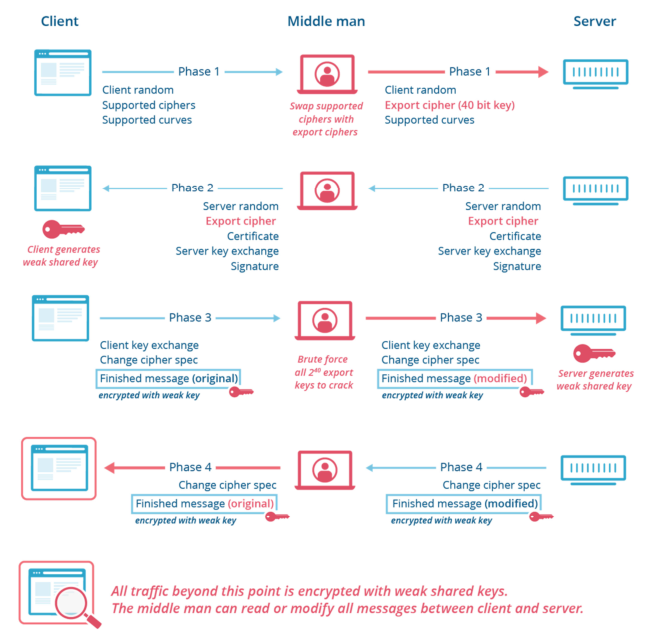
\includegraphics[width=.6\textwidth]{img/FREAK attack.png}
  \caption{FREAK attack.}
  \label{fig:freak-attack}
\end{figure}

\section{ALPN extension}
The ALPN extension, or Application-Layer Protocol Negotiation, is an
extension that allow to negotiate the application protocol to speed up
the connection creation, avoiding additional round-trips for
application negotiation. It is used to negotiate the protocol to be 
used on top of the TLS connection, such as HTTP/2, SPDY, or QUIC,
before the connection is established. This is useful because it saves
time, obviously, because after the connection is established, the
client and server could still fail to communicate because the
application protocol is not supported by the server.\\
The extension is inserted in the client hello message, by setting the
ALPN flag to true and providing a list of supported protocols in the
client HELLO message. The server will respond with the ALPN flag set
to true(if it supports the extension) and the selected protocol.\\
This is also useful for those servers that use different certificates
for the different application protocols.

\section{TLS False Start}
TLS False Start is another extension that allows the client can send
application data together with the ChangeCipherSpec and Finished
messages, in a single segment, without waiting for the corresponding
server messages. The biggest advantage of using this is the reduction
of the latency to 1 RTT. In theory this should work without changes,
but to use this in Chrome and Firefox they require the ALPN and the 
Forward Secrecy enabled, while Safari requires forward secrecy.

\section{The TLS downgrade problem}
In theory, when negotiating the TLS version to be used, the client
sends (in ClientHello) the highest supported version, while the server
notifies (in ServerHello) the version to be used (highest in common
with client).\\
For example if the client support up to SSL 3.3(TLS 1.2) and the
server support the same version, the connection will be established
using TLS 1.2. But if the server supports only SSL 3.2(TLS 1.1), the
connection will be established using SSL TLS 1.1.\\
Some servers, instead of sending the highest version supported, just
close the connection, forcing the client to retry with a lower version
of the protocol. An attacker could exploit this behavior to force the
client to use an older version of the protocol, by repeatedly closing
the connection, and then exploit the vulnerabilities of the older
version of the protocol.\\
\begin{boxH}
  This means that its not a problem of the protocol itself, but of the
  implementation of the server.
\end{boxH}

\subsection{TLS Fallback Signalling Cipher Suite Value (SCSV)}
This behavior is not always an attack, for example there could be and
error in the channel, which is closed by the server. This means that
there's a need to distinguish between a real attack and a simple 
error.\\
The \textbf{TLS Fallback SCSV} is a \textbf{special value} that is
used to prevent the protocol downgrade attacks, not only chiper suite.
It do so by sending a new (dummy) ciphersuite
value(TLS\_FALLBACK\_SCSV) which is sent by the client when opening a
downgraded connection as the last value in the chipersuite list.\\
If the server receives this value and still supports an higher version
of the protocol, it will know that the client is trying to downgrade
the connection, and it will refuse to establish the connection by
sending a \textbf{inappropriate\_fallback} alert message an closing
the channel.\\
This notify the client that he should retry with the highest version 
of the protocol supported by himself.\\
Many servers do no support SCSV yet, but most servers have fixed their
behavior when the client requests a version higher than the supported
one so browsers can now disable insecure downgrade

\section{TLS session tickets}
We know that session resumption is possible with TLS, but the server
needs to keep a cache of session IDs, which may become very large for
high traffic servers. For this reason, the \textbf{TLS session
tickets} were introduced, which are an extension allowing the server
to send the session data to the client encrypted with a server secret
key. This data is stored by the client, which will send it again when
it wants to resume a session. This allows to move the cache to the
client side. Obviously, this data has to be encrypted with a server
secret key.\\
Even if this behaviour is desirable for the server, it still need to
be supported by the browser ( it's an extension after all) and needs a
mechanism to share keys among the servers in a load-balancing heavy
environment.
\section{The Virtual Server Problem}
Nowadays, virtual servers are very common in web hosting, because they
allows to have different logical names associated with the same IP
address( ie: home.myweb.it=10.1.2.3, food.myweb.it=10.1.2.3).
This is easy to manage in HTTP/1.1 but quite troublesome with HTTPS,
because TLS is activated before the HTTP request is sent, which makes
it difficult to know which certificate should be provided in advance.
The solutions are quire simple:
\begin{itemize}
  \item use a wildcard certificate, which is a certificate that is
    valid for all the subdomains of a domain (ie: *.myweb.it)
  \item use the SNI (Server Name Indication) extension, which is an
    extension that allows the client to specify the hostname of the
    server it is trying to connect to, allowing the server to provide
    the correct certificate. This is sent in the ClientHello message.
  \item provide a certificate with a list of servers in
    subjectAltName, which allow to share the same private key for 
    different servers.
\end{itemize}

\section{TLS 1.3}
TLS 1.3 was released in 2018, and it introduced some new features
while solving some of the most common problems of the previous 
versions:
\begin{itemize}
  \item \textbf{reduce} the \textbf{handshake latency} in general 
  \item \textbf{encrypting} more of the \textbf{handshake} (for
    security and privacy, after all up to TLS 1.2 the handshake was in
    clear text)
  \item \textbf{improving resiliency} to cross-protocol attacks
  \item removing legacy features
\end{itemize}
We will now go over the main changes in TLS 1.3.

\subsection{Key exchange}
In this version, the support for static RSA and DH key exchange was
removed for many reasons:
\begin{itemize}
  \item it does not implement forward secrecy 
  \item its difficult to implement correctly, which is a problem
    because it exposes the system to many attacks like Bleichenbacher
\end{itemize}
Now Diffie-Hellman ephemeral (DHE) and Elliptic Curve Diffie-Hellman
Ephemeral (ECDHE) are the only key exchange methods supported, with
some required parameters( some implementations weren't really up to
the standards, ie: used DH with small numbers( just 512 bits) or
generated values without the required mathematical properties).

\subsection{Message protection}
TLS 1.3 greatly improves message protection by eliminating several
vulnerabilities present in earlier versions. Previously, issues arose
from using CBC mode with authenticate-then-encrypt, which led to
attacks like Lucky13 and POODLE. The use of RC4 also allowed plaintext
recovery due to measurable biases, and compression enabled the CRIME
attack.\\
TLS 1.3 addresses these weaknesses by removing CBC mode and enforcing
AEAD modes for stronger security. Insecure algorithms such as RC4,
3DES, Camellia, MD5, and SHA-1 have been dropped, and compression is
no longer used, ensuring a more secure cryptographic environment.

\subsection{Digital signature}
In TLS 1.3, digital signatures have been strengthened to address
earlier vulnerabilities. Previously, RSA signatures were used on
ephemeral keys with the outdated PKCS\#1v1.5 schema, leading to
potential flaws. The handshake was authenticated using a MAC instead
of a proper digital signature, which exposed the protocol to attacks
like FREAK.\\
TLS 1.3 improves this by using the modern, secure RSA-PSS signature
scheme. Additionally, the entire handshake is signed, not just the
ephemeral keys, providing more comprehensive security. The protocol
also adopts modern signature schemes, enhancing the overall strength
of the cryptographic process.

\subsection{Ciphersuites}
TLS 1.3 simplifies the protocol by reducing the complexity seen in
earlier versions, which had a long list of cryptographic options that
grew exponentially with each new algorithm. This complexity made
configuration and security management difficult.\\
To address this, TLS 1.3 specifies only essential, orthogonal
elements: a cipher (and mode) combined with an HKDF hash function. It
no longer ties the protocol to specific certificate types (like RSA,
ECDSA, or EdDSA) or key exchange methods (such as DHE, ECDHE, or
PSK).\\
Moreover, TLS 1.3 narrows the selection to just five ciphersuites:
\begin{itemize}
  \item TLS\_AES\_128\_GCM\_SHA256
  \item TLS\_AES\_256\_GCM\_SHA384
  \item TLS\_CHACHA20\_POLY1305\_SHA256
  \item TLS\_AES\_128\_CCM\_SHA256
  \item TLS\_AES\_128\_CCM\_8\_SHA256 (deprecated but yet supported
    for computational environments with low capacity)
\end{itemize}

\subsection{EdDSA}
\textbf{EdDSA}, or Edwards-curve Digital Signature Algorithm, is a digital 
signature scheme using the EdDSA signature scheme, which is a variant
of the standard elliptic curve DSA schema. The EdDSA scheme,
unlike standard DSA, doesnt require a PRNG, which could in some cases
leak the private key if the underlying generation algorithm is broken
or predictable.\\
EdDSA picks a nonce based on a \textbf{hash of the private key} and
the \textbf{message}, which means after the private key is generated
there’s no need anymore for random number generators. Another
advantage is that the EdDSA is faster in signature generation and
verification than the standard DSA, because it implements simplified
point addition and doubling.\\
EdDSA is using an n-bit private and public keys and will generate a
signature which has a size which is the double of the keys size.
As per the RFC stipulations, EdDSA must support the Ed25519 and
Ed448 curves, which are based on the Edwards-curve Digital Signature,
which uses respectively SHA-2 and SHA-3 as hash functions. Among those
two, Ed25519 is the most used, which is also used for an
implementation of EcDH.\\
When it comes to the RFCs there's an issue: there are two RFCs that 
are slightly different, one is the RFC 8032, which is for general
internet implementations, with the implementational details left to
the developers, and there's also FIPS 186-5, which specifies not only
the mathematics behind an algorithm but also implementation details
because it is a standard for the US government.


\subsection{Other improvements}
TLS 1.3 introduces several key improvements to enhance security and
efficiency. One major change is that all handshake messages sent after
the ServerHello are now encrypted, ensuring better confidentiality
during the handshake process, even if the keys have not been
enstablished(we will go over the details later). The new
\textbf{EncryptedExtensions} message allows additional extensions,
which were previously sent in cleartext during ServerHello, to also
benefit from encryption, improving privacy.\\
Additionally, key derivation functions have been redesigned to support
easier cryptographic analysis due to their clear key separation
properties. HKDF is now used as the underlying primitive for key
derivation, providing a robust and flexible method.\\
The handshake state machine has also been overhauled, making it more
consistent by removing unnecessary messages, such as
\textbf{ChangeCipherSpec}, which is now only retained for
compatibility with older systems. This restructuring streamlines the
handshake process, reducing complexity and improving protocol
efficiency.


\subsection{HKDF in TLS 1.3}
HKDF is one of the novelties of TLS 1.3, and is a HMAC-based
extract-and-expand Key Derivation Function. As a normal key derivation
function, it takes 4 inputs: the salt, the input keying material(
which is basically a secret key), the info string and the output
length. It basically takes the first 2 inputs to derive a key which
will be used to derive a pseudorandom key .Then the second stage
expands this key into several additional pseudorandom keys, which are
the output of the KDF. So multiple outputs can be generated from the
single IKM value by using different values info strings.\\
By calling the function repeatedly call the HMAC function with with PR
keys and the info string as the input message, and then concatenate 
the results, by appending the output of the HMAC function to the 
previous output and incrementing an 8-bit counter.\\
This means that from one call we can generate at most 256($2^8$)
different keys.\\
The finished message is not protected with the master secret as it was
in TLS 1.2, but with the specific key, which is created with expand
starting from the base key and putting as info the text "finished" and
then the desired length. The pre-shared key to protect the ticket
contains the word "resumption". So you start with some basic key
material and then by using different labels, you are able to generate
the different keys.

% add this as a minted pseudocode 
% HKDF-Expand( HKDF-Extract ( salt, IKM ), info, length ) 

\begin{listing}[H]
  \begin{minted}{python}
    HKDF-Expand( HKDF-Extract ( salt, IKM ), info, length )
  \end{minted}
  \caption{HKDF-Expand pseudocode.}
  \label{lst:hkdf-expand}
\end{listing}

\subsection{TLS-1.3 handshake}
Even the handshake in TLS 1.3 was changed. The first thing that we
notice is that the change chiper specs has been removed from the
standard.\\
At first, as you can see from figure \ref{fig:tls-1.3-handshake}, the
connection starts with an hello message from the client, which will
also send it's list of chipersuites. The following message is just the
key share, in which the client will send it's DH parameters(it is
still needed after all).\\ 
The following messages are just the specular ones but sent from the
server this time. After this point it is possible to have
confidentiality of the communication, because a shared key has been
established(the curly braces in the picture are just for that). This
solution allow to save some RTTs, because we can send the needed data
in the HELLO messages.

\begin{figure}[H]
  \centering
  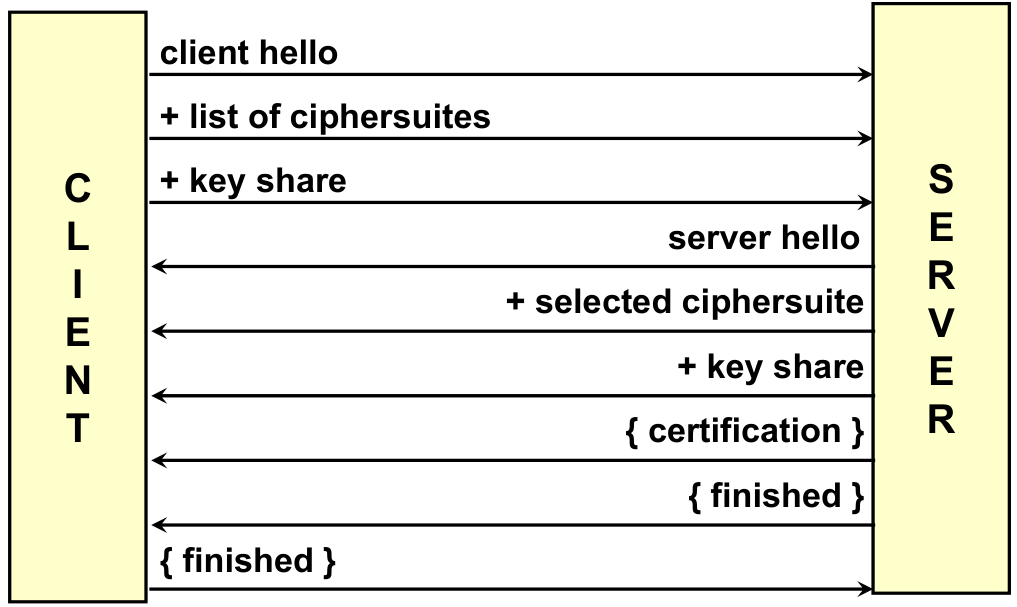
\includegraphics[width=.6\textwidth]{img/TLS 1-3 handshake.png}
  \caption{TLS 1.3 handshake.}
  \label{fig:tls-1.3-handshake}
\end{figure}

\subsection{Pre-shared keys}
In TLS, the pre-shared key (PSK) replaces the session ID and session
ticket. PSKs are agreed upon during a full handshake and can be reused
for multiple connections. They can be combined with (EC)DHE to achieve
forward secrecy, where the PSK is used for authentication and (EC)DHE
for key agreement. While PSKs can be generated out-of-band (OOB) from
a passphrase, this is risky due to the potential lack of randomness,
making brute-force attacks feasible. Therefore, using OOB PSKs is
generally discouraged.

\subsection{0-RTT connections}
In TLS 1.3, when using a pre-shared key (PSK), a client can send
"early data" with its initial message, which is protected by a
specific key. However, this approach lacks forward secrecy because it
relies solely on the PSK and could be vulnerable to replay attacks.
While some complex mitigations exist, they are particularly
challenging for multi-instance servers.

\subsection{Incorrect share}
In TLS 1.3, if a client sends a list of (EC)DHE groups that the server
does not support, the server responds with a HelloRetryRequest,
prompting the client to restart the handshake with different groups.
If the new groups are also unacceptable, the handshake will be
aborted, and the server will send an appropriate alert.

